\documentclass[book.tex]{subfiles}
\begin{document}

\chapter{Multi-dimensional Optimization}
\label{chap:multidimensional}
\noindent\rule{11cm}{0.4pt} \\
\textbf{Prerequisites:} \autoref{chap:newton_raphson} \\
\textbf{Difficulty Level:} * \\
\noindent\rule{11cm}{0.4pt}
\vspace{5mm}

In this chapter, we will learn how to use contour and surface plots to visualize two-dimensional functions. We will then cover how to find local-optima of multi-dimensional functions with gradient descent. 

\section{Multidimensional Optimization}
Aside from one-dimensional functions, optimization also deals with multidimensional functions. Recall from the previous chapters that our visual image of a one-dimensional search was like a roller coaster. For two-dimensional cases, the image becomes that of mountains and valleys.

Techniques for multidimensional unconstrained optimization can be classified in a
number of ways. For purposes of the present discussion, we will divide them depending
on whether they require derivative evaluation. Those that require derivatives are called
gradient, or descent (or ascent), methods. The approaches that do not require derivative evaluation are called non-gradient, or direct, methods. We will be dealing with one of the popular ways of solving multi-dimensional problems using gradients.
\section{Visualizing two-dimensional functions}
\begin{marginfigure}
	\centering
	% 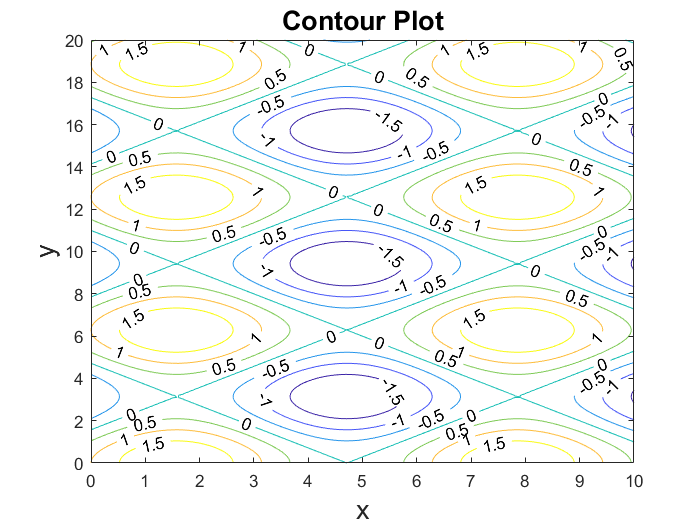
\includegraphics[width = 2.7in]{figures/part1b/multidimensional_optimization/contour.png}
 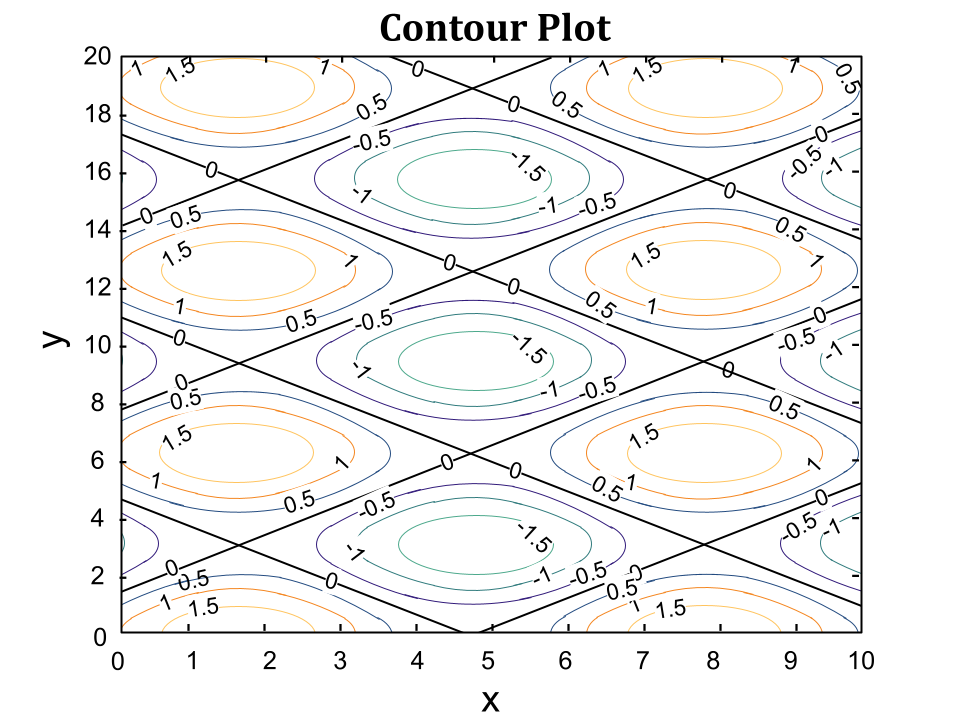
\includegraphics[width = 2.7in]{figures/part1b/multidimensional_optimization/contour0.png}
	\centering
	\caption{Contour plot of the error function}
	\label{fig:1}
\end{marginfigure}

Before delving into optimization, let's look at two popular approaches of visualizing two-dimensional functions namely contour plots and surface plots.

A contour plot is a graphical technique for representing a 3-dimensional surface by plotting constant $f(x,y)$ slices, called contours, on a 2-dimensional format. That is, given a value for $f(x,y)$, lines are drawn for connecting the ($x,y$) coordinates where that $f(x,y)$ value occurs.

Surface plots are diagrams of three-dimensional data. Rather than showing the individual data points, surface plots show a functional relationship between a designated dependent variable $f(x,y)$, and two independent variables $x$ and $y$. The plot is a companion plot to the contour plot.

\begin{marginfigure}
	\centering
	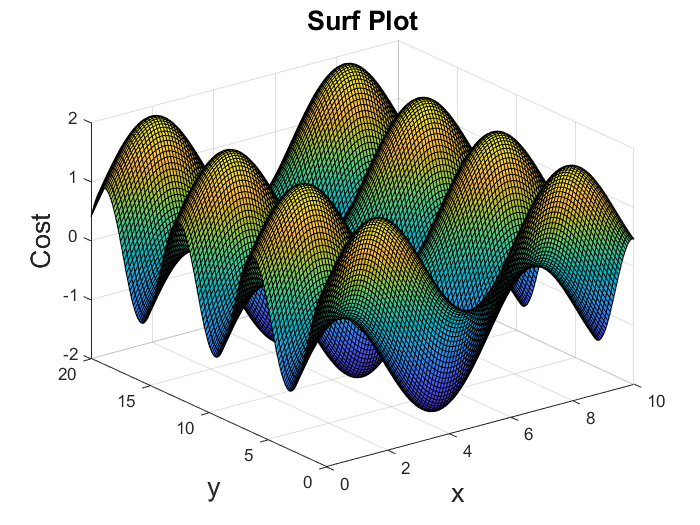
\includegraphics[width = 2.7in]{figures/part1b/multidimensional_optimization/surface.png}
	\centering
	\caption{Surface plot of the Error function}
	\label{fig:2}
\end{marginfigure}

To make this easier to understand, let's look at the surface and contour plots of a function $f(x,y) = \sin(x) + \cos(y)$.  %The plots are obtained by using the \texttt{\textbf{contour}} and \texttt{\textbf{surf}} functions in Matlab.

\section{Gradient-Descent Method}
Let's consider a two-dimensional function $f(x,y)$ depending on the variables $x$ and $y$. It can be observed that most of the two-dimensional functions can be viewed as comprising of mountains and valleys which comprise of local optima.
	
So, let's use the mountain-valley analogy to look at the approach of gradient descent. Suppose that you are lost while trekking, and you have to reach a lake which is at the lowest point of the mountain (a.k.a valley). A twist is that you are blindfolded and you have zero visibility to see where you are headed. The best way is to check the ground near you and observe where the land tends to descend. This will give an idea in what direction you should take your first step. If you follow the descending path, it is very likely you would reach the lake. This is the complete intuition behind gradient descent.
	
Mathematically, this can be interpreted as determining the slope along each dimension and taking a small step in that direction to go down the slope.	The gradient of the two-dimensional function is evaluated as given below:
\begin{align}
\nabla_x &= \frac{\partial f(x,y)}{\partial x}\\
\nabla_y &= \frac{\partial f(x,y)}{\partial y}
\end{align}
	
where $\nabla_x$ is the gradient along x-direction and $\nabla_y$ is the gradient along y-direction. The update rule of gradient descent (i.e taking a step in the gradient direction) is given by
	
\begin{align}
x_{i+1} &= x_{i} - \alpha \nabla_x\\
y_{i+1} &= y_{i} - \alpha \nabla_y
\end{align}
	
where $\alpha$ is the length of the step we want to take down the hill. We can generalize this discussion into a general gradient descent algorithm for $N$ dimensional function.
	
\begin{lstlisting}[language=python]
def gradient_descent(loss: $\mathbb{R}[N] \to \mathbb{R}$, guess: $\mathbb{R}[N]$, $\alpha$ : $\mathbb{R}$, $\epsilon$: $\mathbb{R}$) $\to$ $\mathbb{R}$[N]:
  change = $\infty$
  while change > $\epsilon$:
    gradient = $\nabla$loss(guess)
    new = guess - $\alpha$*gradient
    change = $\|$new - guess$\|$ /$\|$guess$\|$
    if change < $\epsilon$:
      break
    guess = new
  guess
\end{lstlisting}

A simple version of gradient descent is shown above. The relative approximation error between the current guess and the previous guess is chosen for termination. Alternatively, the absolute value of the gradient can also be chosen. This implies that when the gradient is close to zero, we are near an optima and hence can terminate.
	
	
\subsection{Step-Size and Initial Guess}
The step-size variable $\alpha$ controls how large of a step we take downhill during each iteration. If we take too large of a step, we may step over the minimum. However, if we take small steps, it will require many iterations to arrive at the minimum.
	
Another important observation to keep note of is that gradient descent converges to a local optima. This means, in a function with multiple valleys i.e multiple optima, the initial guess (i.e. where we start going down the hill) matters a lot. 
	
Let's look at solving a two-dimensional optimization problem using gradient descent. Suppose a set of measurements are given of the position of a moving particle in one dimension. Let's try to predict the time evolution of the particle by assuming a linear model.

Let's try to fit a linear model to the observed data in the fashion below

\begin{align}
p(t) &= at + b
\end{align}

where $a$ is the velocity of the particle, $b$ is the initial position and $p(t)$ is the position at any given time $t$.

Let's define our loss function to be the least-square error between our model and the data. Let $(t_i,p_i)$ be our data points where $t_i$ is the $i$th time and $p_i$ is the $i$th position. It is given by

\begin{align}
L(a,b) &= \sum_{i=1}^{n}(p_i-(at_i+b))^2
\end{align}

Now, the objective is reduced to find the parameters $a$ and $b$ which minimize the above cost function. To do this, we require the computation of the gradient of the cost function with respect to our parameters. We can use automatic differentiation in general, but for this simple case, we can directly compute gradients to be
\begin{align}
\frac{\partial L}{\partial a} &= -2\sum(p_i-at_i-b)x_i\\
\frac{\partial L}{\partial b} &= -2\sum(p_i-at_i-b)
\end{align}

Using these calculations, we iteratively take steps on the cost function along the gradient direction to obtain the optimal parameters $a$ and $b$.

\begin{lstlisting}[language=python]
def L(a: $\mathbb{R}$, b : $\mathbb{R}$, x: $\mathbb{R}$[N], y: $\mathbb{R}$[N]) $\to$ $\mathbb{R}$:
  cost = 0
  for i: cost += (y[i] - a*x[i] - b)$^2$
  return cost/N

a = Normal(0.8, 1)
b = Normal(2.2, 1)
def regression(x: $\mathbb{R}$[N], y:$\mathbb{R}$[N]) $\to$ $\mathbb{R}$:	
  return gradient_descent(L(x=x, y=y), [a, b], $\alpha$=1e-7, $\epsilon$=1e-8)
\end{lstlisting}


\section{Newton Method}

The principle of using the Newton method for single dimensional optimization can be extended to multi-dimensional functions.  Giving a recap, in the Newton method for optimization of one-dimensional functions, the update rule is given by:
	
\begin{align}
x_{i+1} = x_i - \dfrac{f'(x_i)}{f''(x_i)}
\end{align}
	
This simple update step can be now extended to multi-dimensional functions with continuous second derivatives. Let's take a two dimensional function $f(x,y)$. Now, we have an initial guess of our optima at $x_0$ and $y_0$. The updates of these variables are obtained by independently computing the gradients along the two-dimensions. These update equations are given by:
	
\begin{align}
X_{i+1}  = X_{i} - [Hf(X_i)]^{-1} \nabla f(X_i)
\end{align}

where $X_{i}$ is the guess vector at $i$th iteration and $H$ is the hessian of the function given by 

\begin{align}
Hf(x,y) = 
\begin{bmatrix}
\frac{\partial^2 f}{ \partial x^2} && \frac{\partial f}{\partial x \partial y}\\ \\
\frac{\partial f}{\partial y \partial x} && \frac{\partial^2 f}{\partial y^2}
\end{bmatrix}
ko\end{align}

The partial derivatives in this case are evaluated at the current estimate. Similar approach of computing partial derivatives and iteratively updating the estimates can be done to extend it to higher dimensions.

The intuition for the Hessian comes from the taylor series expansion of multi-dimensional functions. Let's look at the taylor series expansion of $f(x+\delta x,y + \delta y)$ centered at $(x,y)$. This is given by
\begin{align}
f(x+\delta x,y + \delta y) &= f(x,y) + \frac{\partial f}{\partial x}\delta x + \frac{\partial f}{\partial y}\delta y + \frac{1}{2!}(\frac{\partial^2 f}{\partial x^2} \delta x^2 + 2\frac{\partial f}{\partial x \partial y}\delta x\delta y  + \frac{\partial^2 f}{\partial y^2} \delta y^2) + \dots
\end{align}

This equation can be re-written as
\begin{align}
f(X + \delta X) &= f(X) + \nabla f(X)\cdot \delta X + \delta X\cdot H f(X)\cdot\delta X^T  + \dots
\end{align}
  
where $ \nabla f(X)$ is the first order partial derivatives of $f(x,y)$ and $Hf(X)$ is the hessian, which is the second order partial derivatives of $f(x,y)$. Now revisiting the Newton method's update rule, it can be seen that the multi-dimensional update rule is the same as the following one-dimensional update rule
\begin{align}
x_{i+1} = x_i - \dfrac{f'(x_i)}{f''(x_i)} 
\end{align}
 	
with $f'(x)$ corresponding to $\nabla f(X)$ and $f''(x)$ corresponding to  $Hf(X)$.
	
%\section{Matlab Functions for Multi-dimensional Optimization}
%The function \texttt{\textbf{fminunc}} is designed to find the optimum of a multivariable variable function within an initial guess. The fminunc function works as follows. It uses the quasi-newton algorithm by default, which can be modified by adding an \textit{options} parameter to perform gradient descent. It also uses adaptive step-sizing for faster convergence and computes gradients using finite-difference methods.

%\begin{margintable}
%	\textbf{Syntax of \texttt{fminunc}:}
%	\begin{verbatim}
%	[xmin, fval] = fminunc(function,x)
%	\end{verbatim}
%\end{margintable}

%A simple representation of its syntax is \texttt{\textbf{fminunc}(function,x1,x2)}, where \textit{x} and \textit{fval} are the location and value of the minimum, \textit{function} is the name of the function being evaluated, and $x$ is the initial guess of the optima.

%\begin{margintable}
%	\textbf{Displaying iteration details:}
%	\begin{verbatim}
%	options = optimset('display','iter');
%	fminbnd(function,x0,options)
%	\end{verbatim}
%\end{margintable}

%To display additional details about each iteration, optional parameters can be specified using \textit{optimset}. For example, we can display the calculation details as given to the right.\\
%\textbf{Example: } Find the minima of the above-discussed cost function using the Matlab-function \textbf{fminunc} with initial guess of $a = 8$, and $b = -3$.\\
%\textbf{Solution: } 

%\begin{fullwidth}
%	\begin{Verbatim}
%>> Cost = @(x) sum((Stock_2017 - (Time.*x(1) + x(2))).^2)/n;
%>> guess = [0.5;200];
%>> options = optimset('Display','iter','Algorithm','quasi-newton',...
%		'HessUpdate','steepdesc','FinDiffRelStep',1e-10,'MaxFunEvals',500);
%>> guess_matlab = fminunc(Cost,guess,options)
%	\end{Verbatim}
%\end{fullwidth}

%The above commands, when entered in the command-window, displays the result with following attributes:
%\begin{fullwidth}
%	\begin{Verbatim}
%Iteration  Func-count   f(x)        Step-size    
%0           3          2222.46                         
%1           6          1337.35     0.00109571         
%2          18          35.2482     0.00479691       
%3          24          10.9976       0.247981     
%4          36          10.5458     0.00479692
%5          42          10.5374       0.247931   
%6          54          10.5373     0.00479737   
%7          60          10.5373       0.245073     
%8          72          10.5373      0.0048169
% 
% Local minimum found.
% Optimization completed because the size of the gradient is less than the default value
% of the optimality tolerance.
% 
% guess_matlab =
%    0.9349
%    227.6532
%	\end{Verbatim}
%\end{fullwidth}

%Thus, after three iterations, the method switches from golden to parabolic, and after nine iterations, the minimum is determined to a tolerance of 0.0001.
%\end{document}
\section{Exercises}
\begin{enumerate}
    \item Use gradient descent to find an approximate local minima of the function $f(x,y) = \sin(x) + \cos(y)$
    \item Use the Newton method to find an approximate local minima of $f(x, y) = \sin(x) + \cos(y)$
\end{enumerate}
\end{document}